%!TEX TS-program = pdflatex
%!TEX encoding = UTF-8 Unicode

\documentclass[11pt]{article}
\usepackage{jeffe,handout,graphicx,mathtools}
\usepackage[utf8x]{inputenc}			% allow Unicode in .tex file
\usepackage{enumerate}
\usepackage{fourier-orns}

\def\Sym#1{\texttt{\upshape\textcolor{BrickRed}{#1}}}
\def\SymBlue#1{\texttt{\upshape\textcolor{RoyalBlue}{#1}}}
\def\SymGreen#1{\texttt{\upshape\textcolor{PineGreen}{#1}}}
\def\_#1{\SymBlue{\underline{\smash{\textbf{#1}}}}}
\def\X#1{\SymGreen{$\overline{\textbf{#1}}$}}
\def\u#1{\raise0.5ex\hbox{\textcolor{RoyalBlue}{#1}}}

\def\Cdot{\mathbin{\text{\normalfont \textbullet}}}

\newcommand{\IsSinL}{\text{IsStringInL}}

% =========================================================
\begin{document}

\headers{CS/ECE 374}{Homework 8 (due April 5)}{Spring 2017}

\thispagestyle{empty}

\begin{center}
\Large\textbf{CS/ECE 374 \,\decosix\,  Spring 2017}%
\\
\LARGE\textbf{\decothreeleft~ Homework 8 ~\decothreeright}%
\\[0.5ex]
\large Due Wednesday, April 5, 2017 at 10am
\end{center}

\bigskip
\hrule
\bigskip

\noindent
\textbf{Groups of up to three people can submit joint solutions.}  Each problem should be submitted by exactly one person, and the beginning of the homework should clearly state the Gradescope names and email addresses of each group member.  In addition, whoever submits the homework must tell Gradescope who their other group members are.
\bigskip
\hrule
\bigskip


\noindent
The following unnumbered problems are not for submission or grading. 
No solutions for them will be provided but you can discuss them on Piazza.
\begin{itemize}
\item In the lab you saw how to compute $s$-$t$ shortest walks
efficiently when the graph has a single negative length edge. The running
time is asymptotically the same as using Dijkstra's algorithm. Generalize
this to the setting where the graph has {\em two} negative length edges.

\item See HW 8 problems from Fall 2016 available at 
\url{https://courses.engr.illinois.edu/cs374/fa2016/homework/hw8.pdf}.
\item Given a directed graph $G=(V,E)$ with non-negative edge lengths,
and two nodes $s,t$, the bottlenect length of a path $P$ from
$s$ to $t$ is the maximum edge length on $P$. The bottleneck distance
from $s$ to $t$ is defined to be the smallest bottleneck path legnth
among all paths from $s$ to $t$. Describe an algorithm to compute
the bottleneck shortest path distances from $s$ to every node in $G$
by adapting Dijkstra's algorithm. Can you also do it via a reduction
to the standard shortest path problem?
\end{itemize}

\vspace{1cm}

\begin{enumerate}
%\parindent 1.5em \itemsep 3ex plus 0.5fil

%----------------------------------------------------------------------
%\def\arraystretch{1.2}

%----------------------------------------------------------------------
\item Let $G = (V, E)$ be a connected directed graph with non-negative
  edge weights, let $s$ and $t$ be vertices of $G$, and let $H$ be a
  subgraph of $G$ obtained by deleting some edges.  Suppose we want to
  reinsert exactly one edge from $G$ back into $H$, so that the
  shortest path from $s$ to $t$ in the resulting graph is as short as
  possible. Describe and analyze an algorithm that chooses the best
  edge to reinsert. Ideally the running time of your algorithm should
  be {\em asymptotically} the same as that of running Dijkstra's algorithm.

%----------------------------------------------------------------------
\item Let $G=(V,E)$ be a directed graph. Describe a linear-time algorithm
that given $G$, a node $s \in V$ and an integer $k$ decides whether
there is a {\em walk} in $G$ starting at $s$ that visits at least $k$ distinct
nodes. The following questions may help you.
\begin{itemize}
\item What is the answer if $G$ is strongly connected?
\item How would you solve the problem if $G$ is a DAG?
\end{itemize}

%----------------------------------------------------------------------
\item Let $G=(V,E)$ a directed graph with non-negative edge
  lengths. Let $R \subset E$ and $B \subset E$ be red and blue edges
  (the rest are not colored).  Given $s,t$ and integers $h_r$ and
  $h_b$ describe an efficient algorithm to find the length of a
  shortest $s$-$t$ path that contains at most $h_r$ red edges and at
  most $h_b$ blue edges.
\end{enumerate}

\vspace{1in}
\subsection*{Solved Problem}

\begin{enumerate}
\Hard
\item[4.]
Although we typically speak of “the” shortest path between two nodes, a single graph could  contain several minimum-length paths with the same endpoints.  

\begin{center}\footnotesize\sffamily
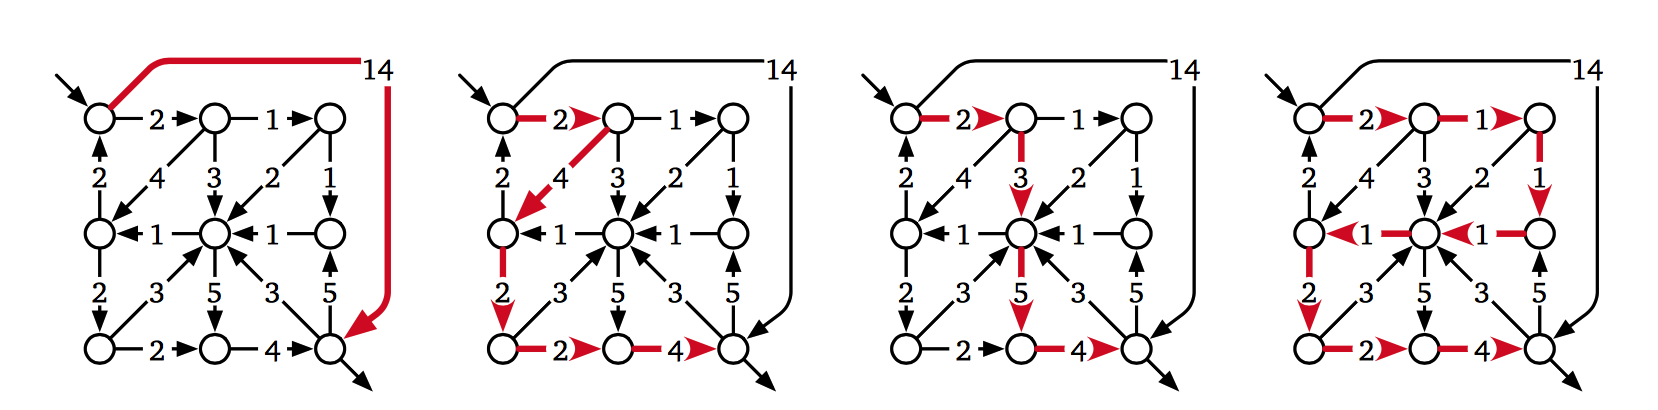
\includegraphics[scale=0.4]{Fig/three-shortest-paths}\\
Four (of many) equal-length shortest paths.
\end{center}

Describe and analyze an algorithm to determine the \emph{number} of shortest paths from a source vertex $s$ to a target vertex $t$ in an arbitrary directed graph $G$ with weighted edges.  You may assume that all edge weights are positive and that all necessary arithmetic operations can be performed in $O(1)$ time.  

\Hint{Compute shortest path distances from $s$ to every other vertex.  Throw away all edges that cannot be part of a shortest path from $s$ to another vertex.  What’s left?}


\begin{solution}
We start by computing shortest-path distances $\emph{dist}(v)$ from $s$ to $v$, for every vertex $v$, using Dijkstra’s algorithm.  Call an edge $\arc{u}{v}$ \EMPH{tight} if $\emph{dist}(u) + w(\arc{u}{v}) = \emph{dist}(v)$.  Every edge in a shortest path from $s$ to $t$ must be tight.  Conversely, every path from $s$ to $t$ that uses only tight edges has total length $\emph{dist}(t)$ and is therefore a shortest path!

Let $H$ be the subgraph of all tight edges in $G$.  We can easily construct $H$ in $O(V+E)$ time.  Because all edge weights are positive, $H$ is a directed acyclic graph.  It remains only to count the number of paths from $s$ to $t$ in $H$.

For any vertex $v$, let $\emph{PathsToT}(v)$ denote the number of paths in $H$ from $v$ to $t$; we need to compute $\emph{PathsToT}(s)$.  This function satisfies the following simple recurrence:
\[
	\emph{PathsToT}(v) = 
	\begin{cases}
		1 & \text{if $v = t$}\\[0.5ex]
		\displaystyle \Sum_{\arc{v}{w}}^{~} \emph{PathsToT}(w) & \text{otherwise}
	\end{cases}
\]
In particular, if $v$ is a sink but $v\ne t$ (and thus there are no paths from $v$ to $t$), this recurrence correctly gives us $\emph{PathsToT}(v) = \sum\varnothing = 0$.

We can memoize this function into the graph itself, storing each value $\emph{PathsToT}(v)$ at the corresponding vertex $v$.  Since each subproblem depends only on its successors in $H$, we can compute $\emph{PathsToT}(v)$ for all vertices $v$ by considering the vertices in reverse topological order, or equivalently, by performing a depth-first search of $H$ starting at $s$.  The resulting algorithm runs in $O(V+E)$ time.

The overall running time of the algorithm is dominated by Dijkstra’s algorithm in the preprocessing phase, which runs in \EMPH{$O(E\log V)$ time}.
\end{solution}

\begin{rubric}
10 points = 5 points for reduction to counting paths in a dag + 5 points for the path-counting algorithm (standard dynamic programming rubric)
\end{rubric}

\end{enumerate}

\end{document}
